\chapter{Three Pinyin Input Methods}
\label{c:prototypes}


We have designed and implemented 3 Chinese keyboards for circular smartwatches. Figure \ref{fig:figure1} shows our three prototypes. Each prototype has been implemented natively for Android Wear 2.0 and tested on an LG Watch Style. This smartwatch has a round 1.2" (30 mm) screen. Our implementation is open-source software, so that other researchers or developers can reuse and build upon our code.\footnote{https://github.com/rednoah/android-wear-pinyin}




\section{Growing Finals}
The Growing Finals keyboard (Figure \ref{fig:figure1}a) exploits an intrinsic characteristic of the Pinyin romanization system: out the 26 letters of the Latin alphabet, 23 can appear as the first letter in a Pinyin syllable, while the remaining 0 to 4 Latin letters of any Pinyin syllable are composed from only 9 unique Latin characters. Liu, et al. have previously exploited this characteristic in PinyinPie \cite{Liu:2012:PPM:2371574.2371614}.
Further research revealed that after selecting the first letter from a list of 23 options is entered, entering the remaining letters of any Pinyin syllable requires no more than 6 unique possible next letters (including the syllable separator \' if necessary) in any input state.
Hence, the Growing Finals keyboard will present a full QWERTY keyboard in its initial state and the---depending on the input---adapt and enlarge possible next letters while preserving the general QWERTY layout (Figure \ref{fig:figure2}). This allows for significantly larger keys after entering the initial letter for each syllable and thus improved input speed and accuracy according to Fitts' law.





\begin{figure}
  \centering
  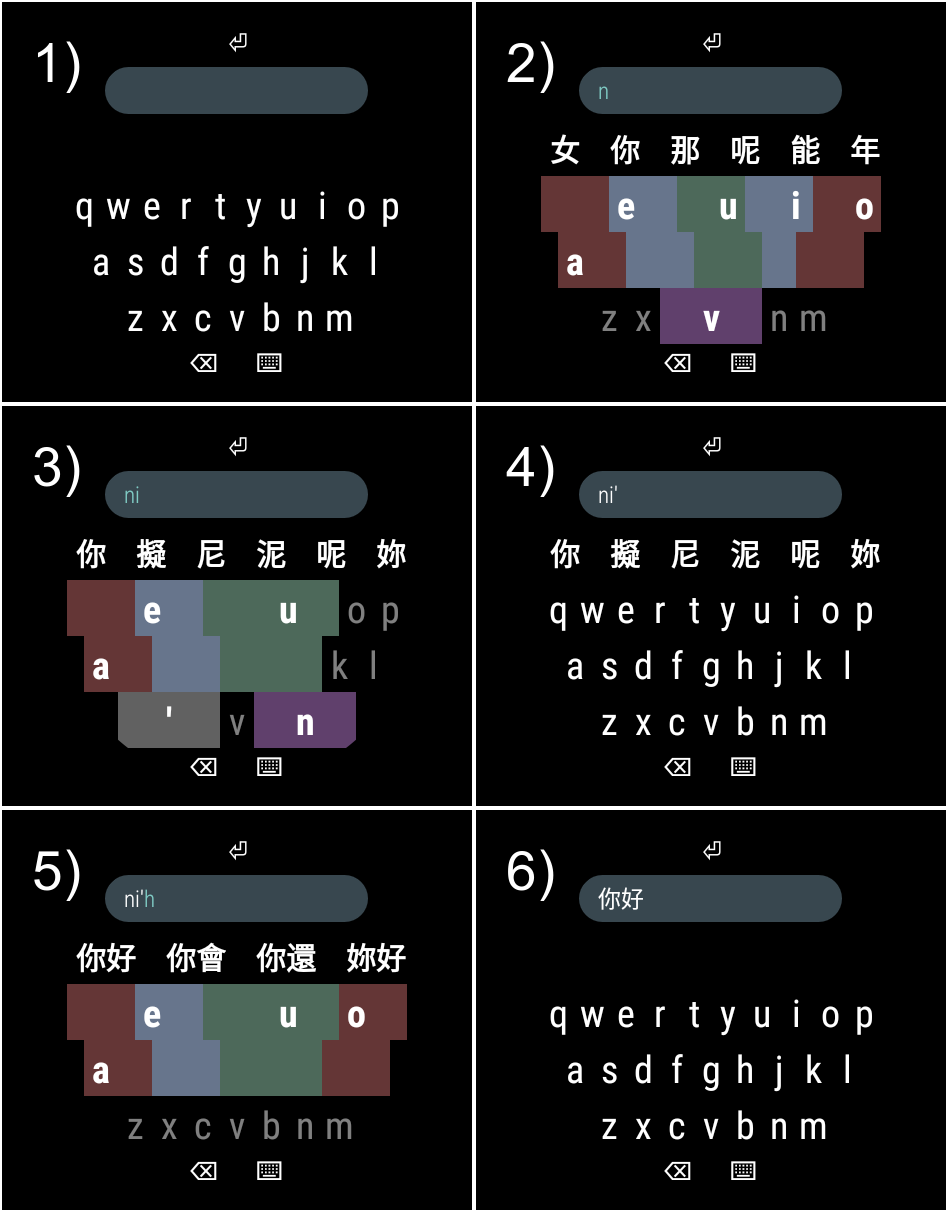
\includegraphics[width=1\columnwidth]{figures/sequence_GrowingFinals}
  \caption{Input sequence for the word 你好 (Pinyin: nǐ hǎo) using Growing Finals: 1) Press n 2) Press i 3) Press ‘詞 4) Press h 5) Select 你好}~\label{fig:figure2}
\end{figure}






\section{Pinyin Syllables}
Each Pinyin syllable can be seen as a combination of an initial sound and a final sound. Initials with similar sounds (e.g., b and p) tend to be combined with a similar set of final sounds (e.g., bang and pang) due to language characteristics. An analysis of the language model reveals that for each of the 26 initial sounds, there are between 2 and 24 (\textit{M} = 15.4, \textit{SD} = 5.6) possible final sounds (including no final sound for vowels such as a and e).
The Pinyin Syllables input method implements a 2-stage design based on Pinyin initials and finals which allows users to enter any Pinyin syllable with exactly 2 keystrokes. The first stage uses a pseudo-QWERTY keyboard layout to leverage existing familiarity with the standard QWERTY keyboard layout. The u, i, and v keys have been removed, and keys for sh, zh, and ch have been added so that each key on the initial keyboard corresponds to exactly one initial sound. Once an initial key has been entered, the keyboard will adapt and display all possible finals for the current input state (Figure \ref{fig:figure3}). Helping with visual search, finals with similar sounds are grouped by colour and placed near corresponding QWERTY keys if possible. Depending on the entered initial, the second stage may contain between 2 and 24 buttons allowing for significantly larger buttons in most cases with the added benefit that a single key press that completes the pinyin syllable may correspond to more than one Latin letter.





\begin{figure}
  \centering
  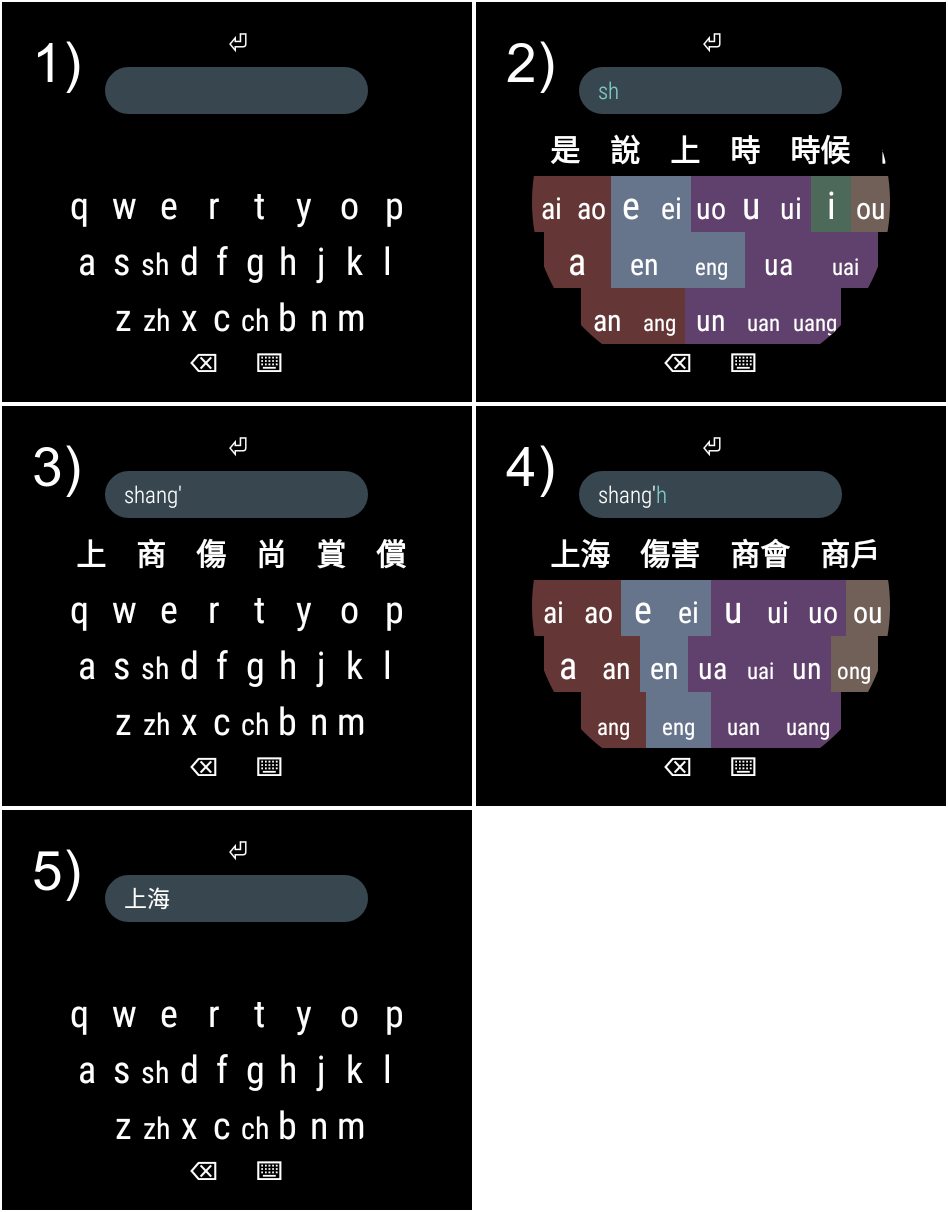
\includegraphics[width=1\columnwidth]{figures/sequence_PinyinSyllables}
  \caption{Input sequence for the word 上海 (pinyin: shàng hǎi) using Pinyin Syllables: 1) Press sh 2) Press ang 3) Press h 4) Select 上海}~\label{fig:figure3}
\end{figure}







\section{Standard QWERTY}
We implement the standard QWERTY keyboard with support for Chinese character entry (Figure \ref{fig:figure1}c) in addition to our two novel input methods to serve as a baseline for comparison. This keyboard design is used by almost all native speakers from China and language students from abroad that type Chinese characters on a computer and thus very familiar to most user.




\section{Common Features}
Each keyboard has a text field that shows the text that has been entered so far. Partial Pinyin input that defines the current state of the keyboard is highlighted. Selecting Chinese characters from the list of suggested candidates will replace the current Pinyin input with the selected Chinese characters and reset the keyboard to its original state for the next input sequence. The rotating hardware button can be used to scroll through the list of Chinese character suggestions without occluding the screen. The DELETE key can be used to delete the most recently entered Latin letter or Chinese character. Cursor movements are not supported.

We use the cross-platform native library RIME \cite{rime} as high-performance Pinyin-to-Chinese-Character conversion engine via Java Native Interface (JNI) on our Android Wear prototype. RIME uses state-of-the-art language models and algorithms with support for intelligent character level, phrase level and full sentence level Chinese character prediction based on complete or partial Pinyin sequences.
